The proposed solution technique is designed to be implemented at the point of common coupling (PCC) of a microgrid containing distributed generation (DG) and energy storage (ES). Fig. \ref{fig:system_arch} depicts an example system. Here, the energy storage management system (ESMS) is in charge of controlling the battery connected to the grid with the objective of getting the most cost optimum use of the resources available. The objective of the ESMS is to optimize the use cost of energy storage under different pricing schemes by taking advantage of RTP or time of use (TOU) prices, load and DG generation forecasting.  Fig. \ref{fig:F1_CA} shows the top-level architecture of the ESMS. As seen in the figure, the inputs of the system are the real-time price (RTP) prediction, load prediction, and the DG prediction, which in this case is a photovoltaic (PV) plant. It will also consider the current state of the load, PV generation, and ES. The output of the ESMS is the optimum battery charge and discharge control references based on the current and forecasted data.

\begin{figure}[!htbp]
\centering
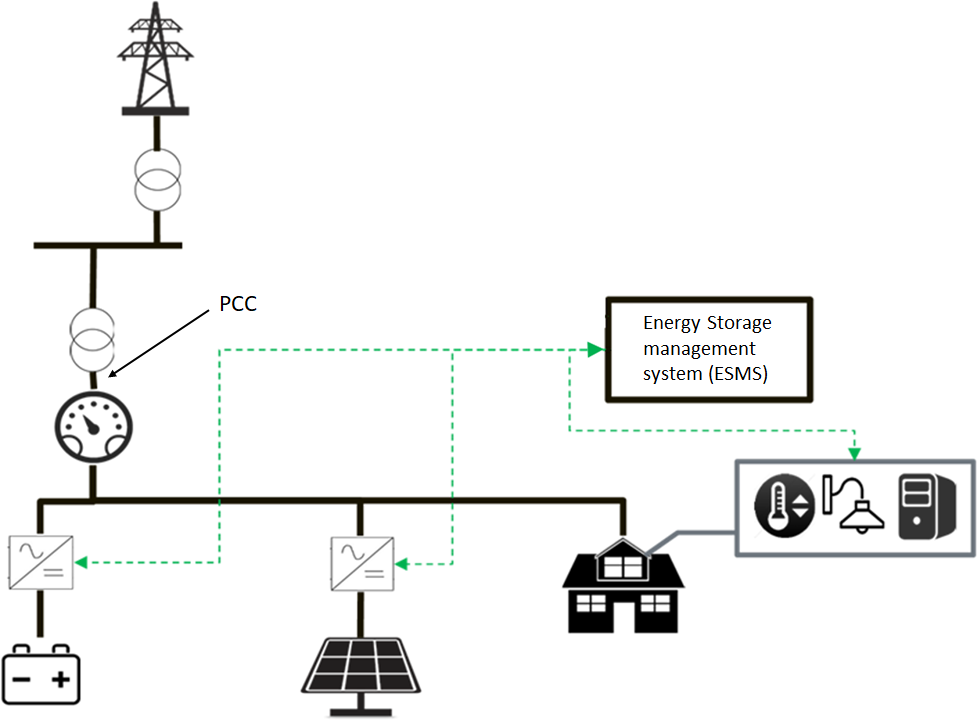
\includegraphics[width=\linewidth]{figs/System_architecture.png}
\caption{Test system architecture}
\label{fig:system_arch}
\vspace{-3mm}
\end{figure}

%  Fig. \ref{fig:F1_CA} shows the top-level architecture of the ESMS. As seen in the figure, the inputs of the system are the real-time price (RTP) prediction, load prediction, and the DG prediction, which in this case is a photovoltaic (PV) plant. It will also consider the current state of the load, PV generation, and ES. The output of the ESMS is the optimum battery charge and discharge control references based on the current and forecasted data.

\begin{figure}[!ht]
    \centering
    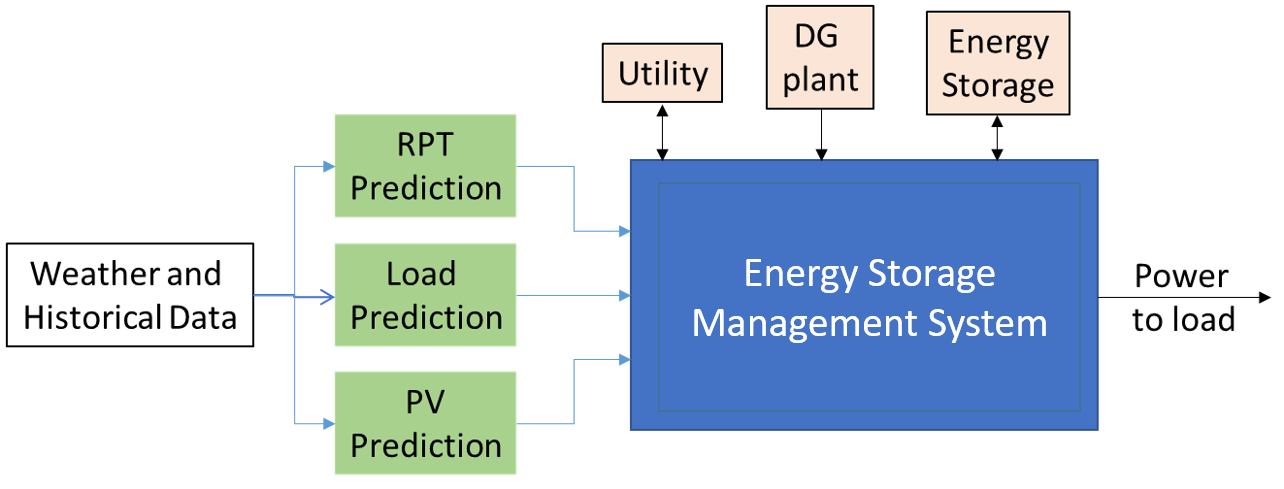
\includegraphics[width = \linewidth]{figs/EMS_FIG.png}
    \caption{Controller top level architecture}
    \label{fig:F1_CA}
\end{figure}

In order to find the optimum cost solution based on the current status of the system and future forecasts, the optimization problem is formulated using a graph search problem approach. To represent the solution space of the problem as a graph, the state of charge (SOC) of the ES, and both the prediction horizon and the control horizon are discretized. Fig. \ref{fig:F1_Dis} demonstrates an example of the discretized solution space.

\begin{figure}[!ht]
    \centering
    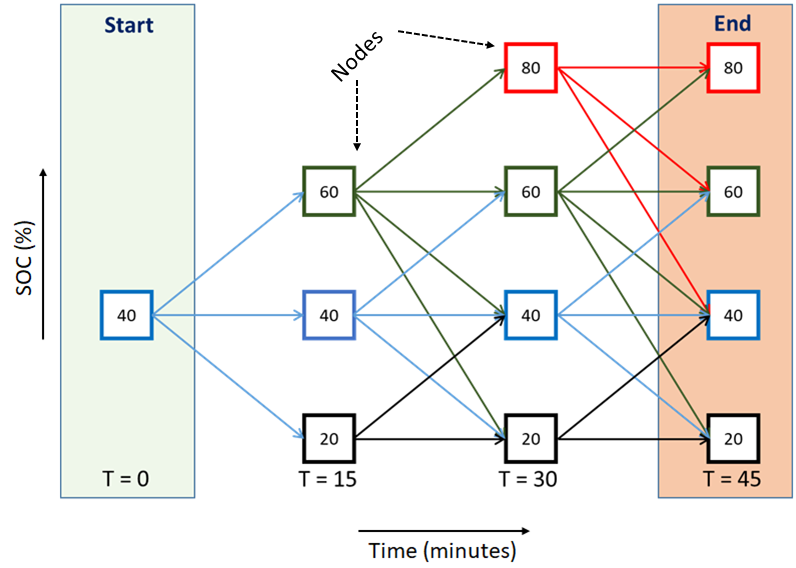
\includegraphics[width = \linewidth]{figs/F1_1_Dis.png}
    \caption{Discretizing solution space}
    \label{fig:F1_Dis}
\end{figure}

The horizontal axis of the figure represents time, and the vertical axis represents discrete steps in the state of charge (SOC) of the energy storage. In this simple example scenario, it is assumed that the algorithm recalculates the solution every 15 minutes (control horizon) based on available data. The SOC of the energy storage system (ESS) is discretized in steps of 20\%, and the SOC is limited between 80\% and 20\%. It is also assumed that the ESS can discharge a maximum of 40\% of its maximum SOC and charge a maximum of 20\% of its SOC in a 15 minute time step. These values are chosen arbitrarily in this simple example scenario to explain the problem. Taking these features into consideration, a directed graph is constructed looking ahead three time steps into the future. The square boxes represent nodes on the graph. The numbers inside the boxes represent the SOC of the ESS at that node. The arrows from the boxes represent all the possible states the ESS can be in the next time step according to the constraints of the system. The arrows are treated as edges of the graph. In this case, the edges are unidirectional. The goal is to find the most cost efficient path to reach T = 45 minute.


